\documentclass[addpoints]{exam}

\usepackage{amsmath,amssymb,amsthm}
\usepackage{graphicx}
\usepackage{hyperref}
\usepackage{tabularx}

\graphicspath{{images/}}

\theoremstyle{definition}
\newtheorem{definition}{Definition}[section]

\theoremstyle{claim}
\newtheorem{claim}{Claim}

\title{Quiz 6: Proofs}
\author{CS/MATH 113 Discrete Mathematics L1}
\date{Habib University | Spring 2023}


\runningheader{}{}{}
\runningfooter{}{}{}

% solution
\usepackage{draftwatermark}
\SetWatermarkText{Sample Solution}
\SetWatermarkScale{3}
\printanswers

\newcolumntype{L}{>$l<$}

\begin{document}
\maketitle
\thispagestyle{empty}

\noindent
\begin{tabularx}{\linewidth}{Xr}
  Total Marks: \numpoints & Date: \today\\
  Duration: 15 minutes & Time: 1715--1730h
\end{tabularx}
\hrule
\bigskip

\noindent \textbf{Student ID}: \hrulefill \\[5pt]
\noindent \textbf{Student Name}: \hrulefill \\[5pt]

% \section{Problems}

\begin{questions}
  \question [10]

  \begin{quotation}
The Pythagoreans were an ancient group of mathematicians and philosophers that lived around the 6th century BC in Greece. They were lead by Pythagoras and very little is known about them, with none of their writings surviving. A lot of mythology is build up around them, including such things as Pythagoras being all knowing, traveling through time and space, and having mystical powers. They supposedly believed a bunch of weird stuff, like the musical scales having mystic properties, and not being able to eat beans (with a wide variety of reasons given by different accounts, even stuff like that you would lose part of your soul when you farted). One story about them is that Pythagoras murdered his student, Hippasus, for discovering irrational numbers (numbers which cannot be expressed as a ratio of two integers). The proof in the comic is for the square root of two (sometimes it is the golden ratio in the story), and is probably not the one discovered by the Pythagoreans, since they aren't known to have algebraic proofs. The Pythagorean Theorem, which is related, was proven with geometry.    
  \end{quotation}
  \hfill --- \href{https://existentialcomics.com/comic/189}{Comic 189, Existential Comics}
  
  Consider the proof provided by Hippasus on the following pages.
  \begin{parts}
    \part Out of the proof techniques that we have studied, which one is Hippasus using?
    \part Justify your claim above. That is, explain why you claim the proof to be of the type that you mention above.
  \end{parts}
  
  \begin{solution}
    \begin{parts}
      \part This is a proof by contradiction.
      \part Hippasus shows that the assumption that $\sqrt{2}$ is irrational leads to the contradiction that $\frac{P}{Q}$ is a non-reducable ratio, as well as a reducable one. Based on this, he concludes that the assumption is false, i.e. $\sqrt{2}$ is rational.
    \end{parts}
  \end{solution}

  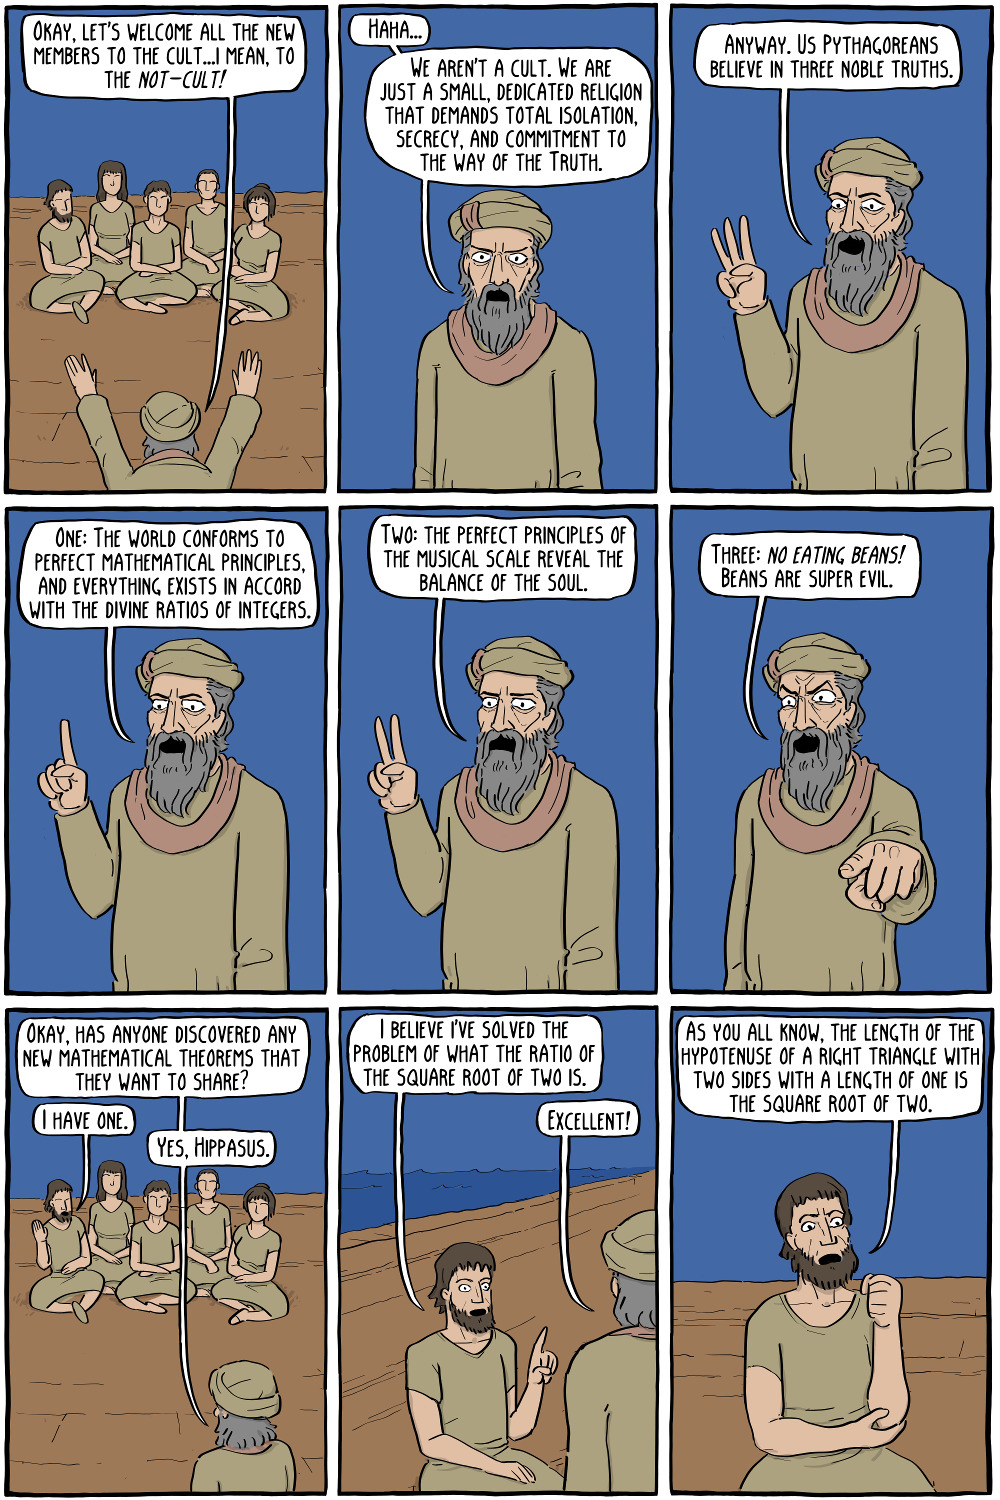
\includegraphics[width=\textwidth]{pyth1}
  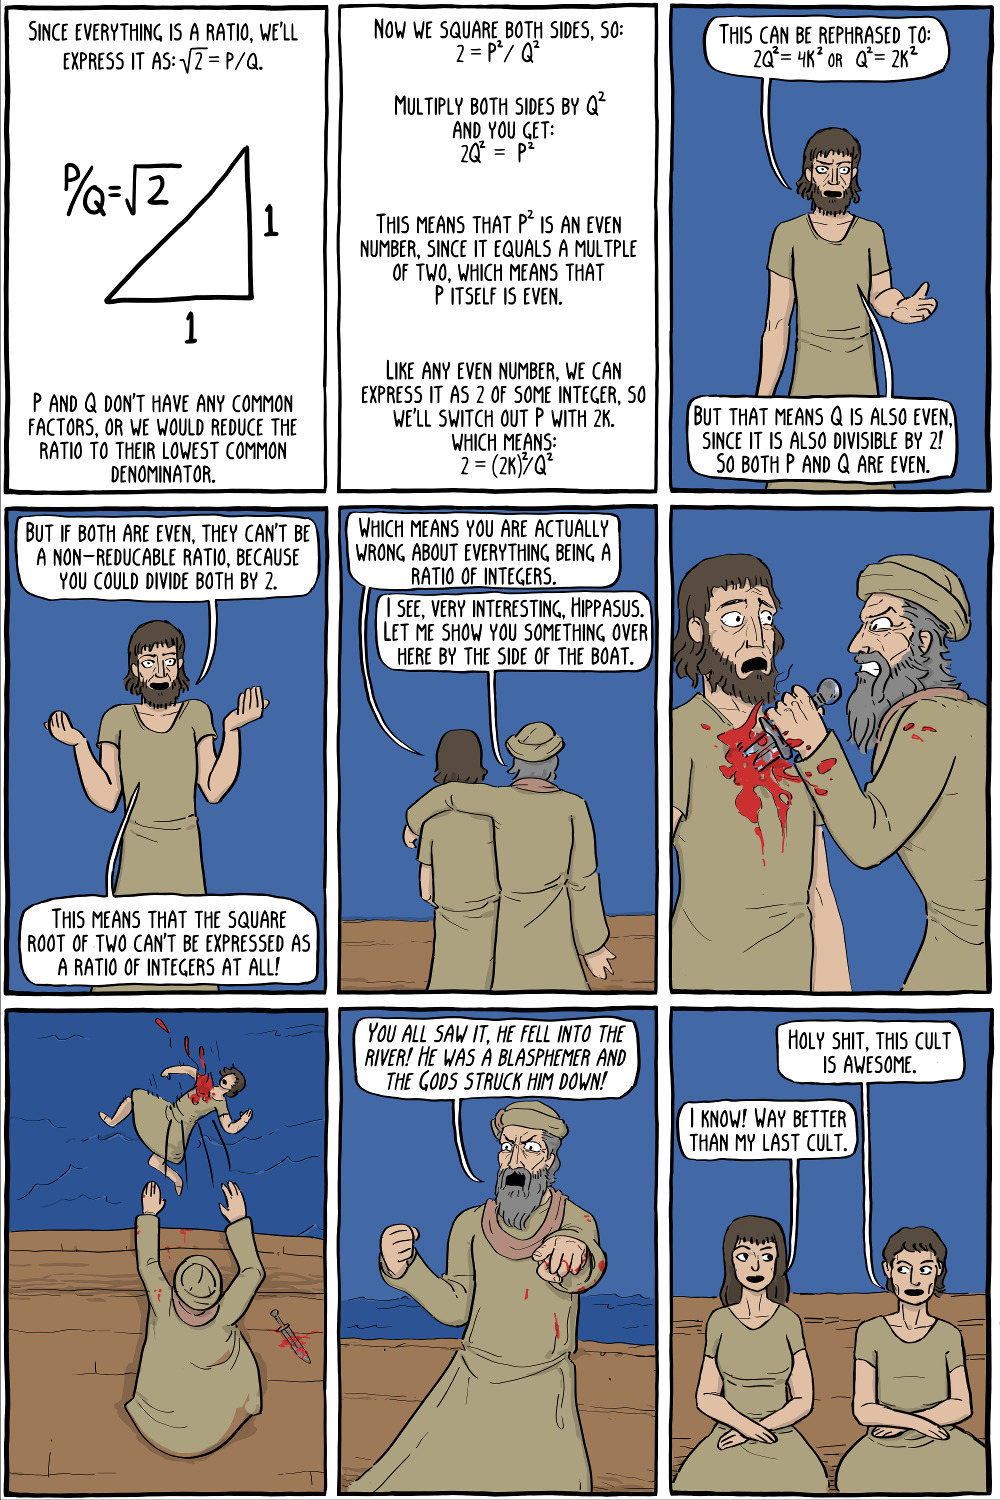
\includegraphics[width=\textwidth]{pyth2}
\end{questions}
\end{document}

%%% Local Variables:
%%% mode: latex
%%% TeX-master: t
%%% End:
